% !TeX root = ../Notizen.tex
\section*{Aufgabe 2: Poincaré Schnitt}
\subsection*{a)}
Die Phasenraumbilder für die drei betrachteten Fälle sind in \cref{fig:phasenraum1,fig:phasenraum2,fig:phasenraum3} dargestellt.
\begin{figure}[h!]
	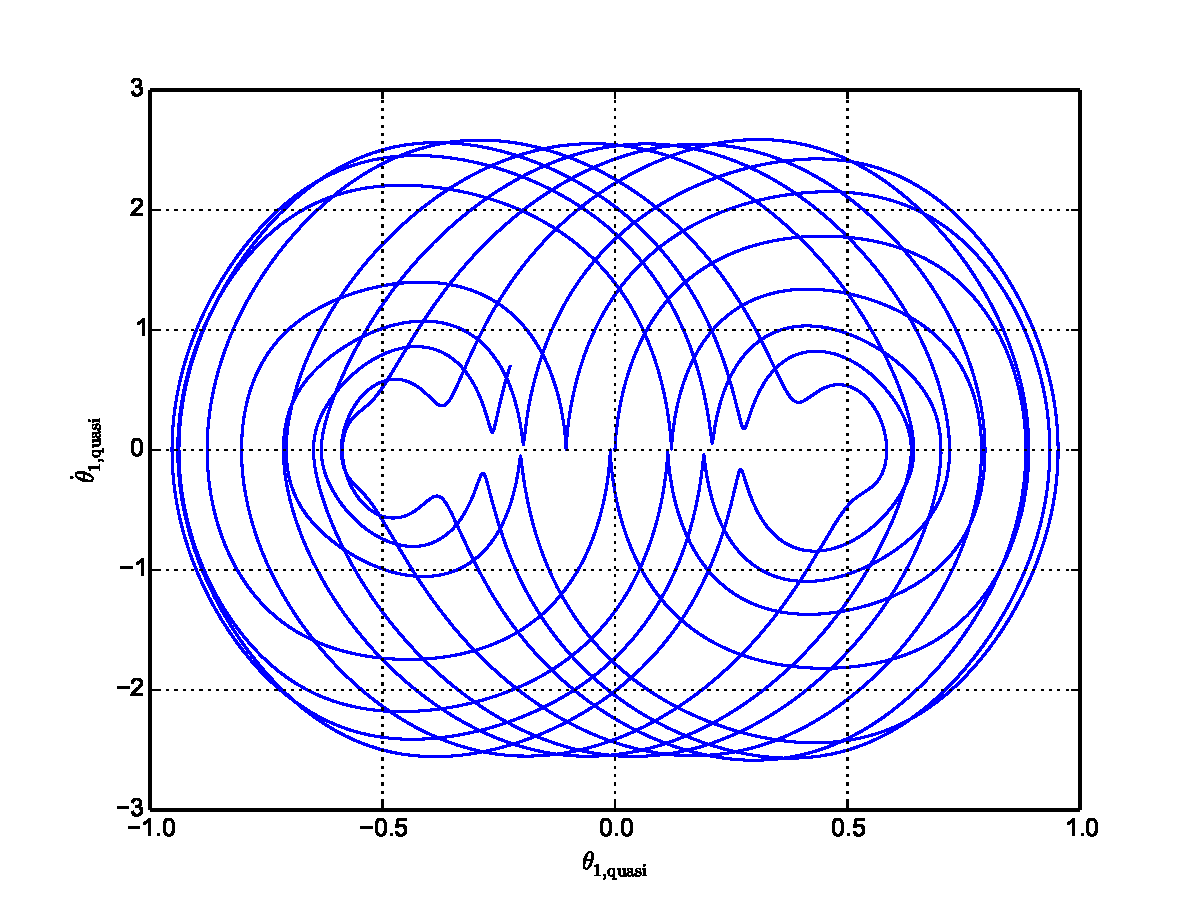
\includegraphics[width = \textwidth]{../Plots/Plot_2_A_1_Phasenraum.pdf}
	\caption{Phasenraum für quasiperiodisches Verhalten.\label{fig:phasenraum1}}
\end{figure}

\begin{figure}[H]
	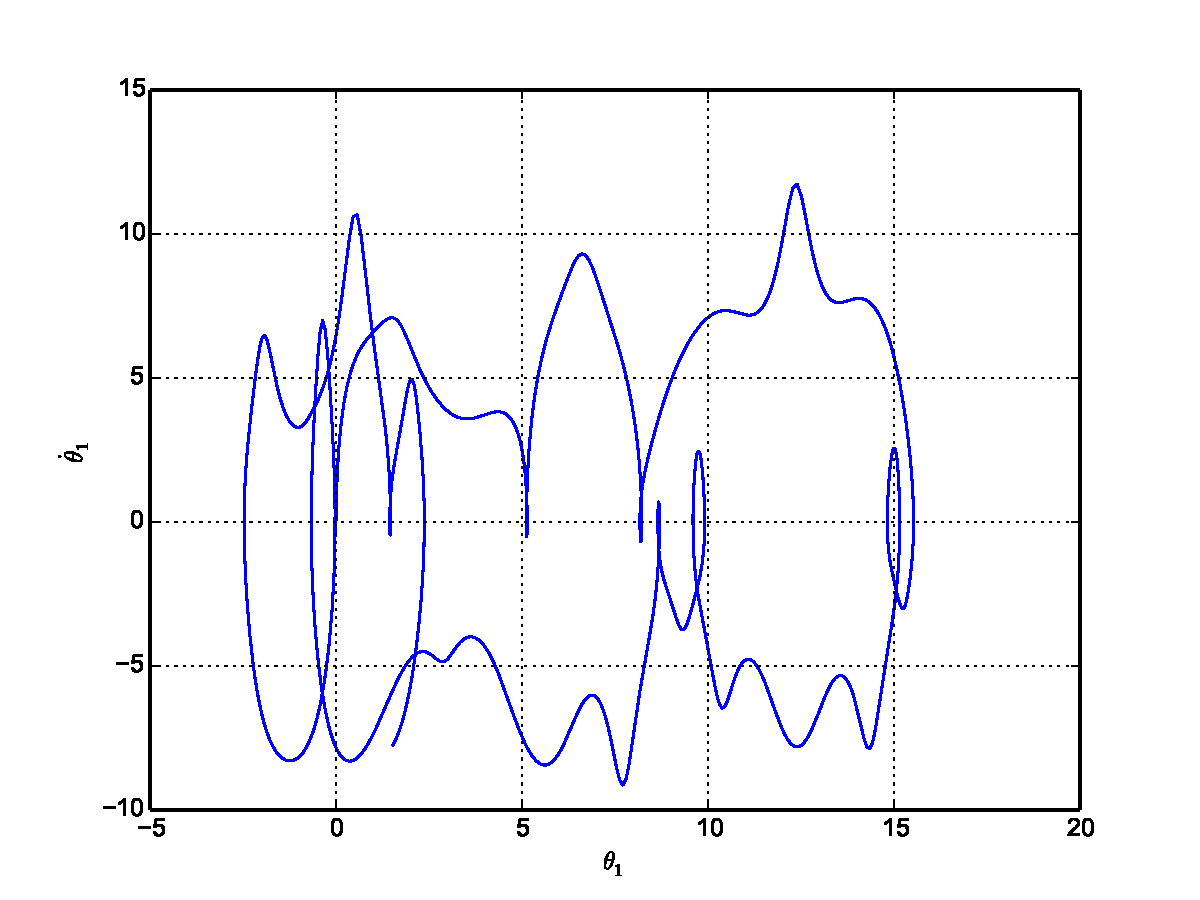
\includegraphics[width = \textwidth]{../Plots/Plot_2_A_2_Phasenraum.pdf}
	\caption{Phasenraum für chaotisches Verhalten.\label{fig:phasenraum2}}
\end{figure}

\begin{figure}[H]
	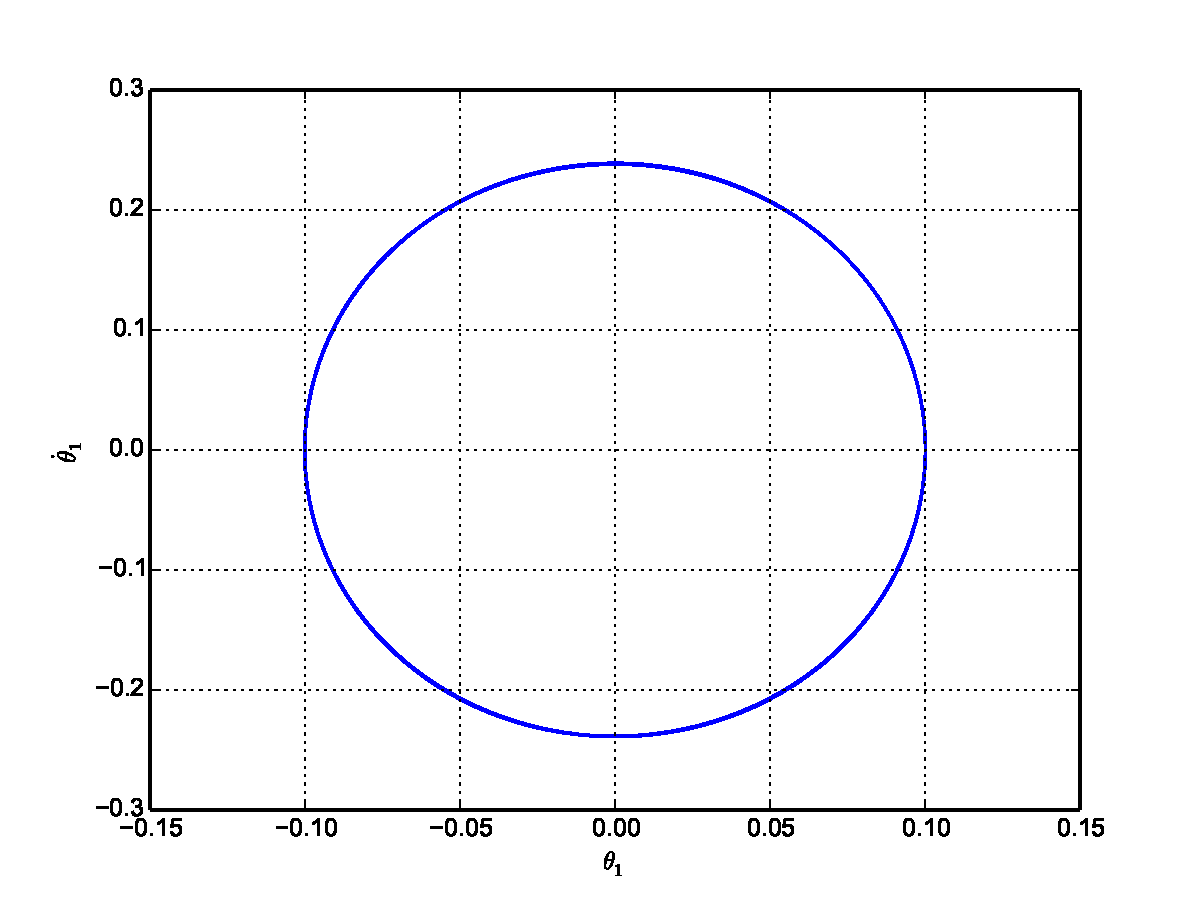
\includegraphics[width = \textwidth]{../Plots/Plot_2_A_3_Phasenraum.pdf}
	\caption{Phasenraum für periodisches Verhalten ($\theta_2=\sqrt{2}\theta_1$).\label{fig:phasenraum3}}
\end{figure}

\newpage\newpage
\subsection*{b)}
Der Abstand der quasiperiodischen Schwingung von der ungestörten ist in \cref{fig:abstand1} dargestellt.
\begin{figure}[H]
	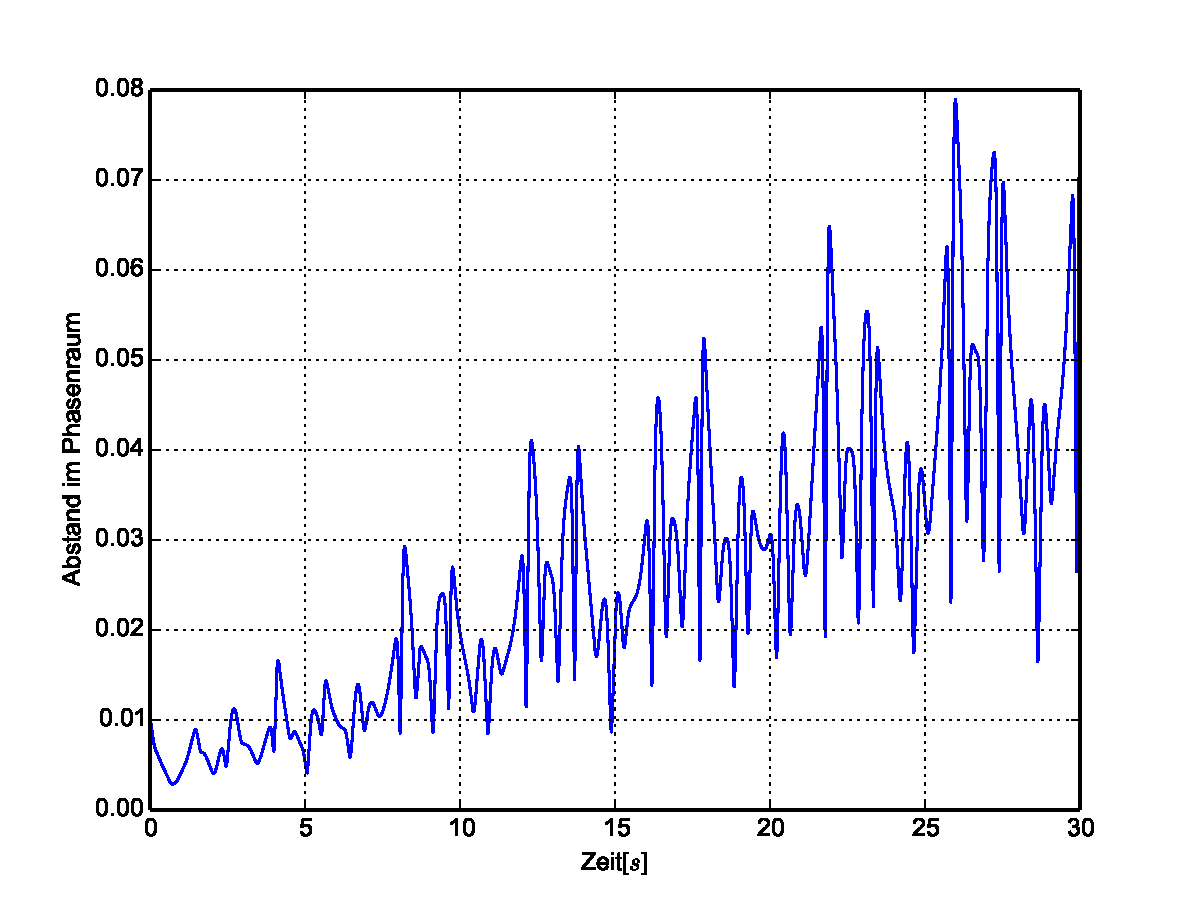
\includegraphics[width = \textwidth]{../Plots/Plot_2_B_1.pdf}
	\caption{Abstand der Trajektorie der quasiperiodischen Schwingung von der ungestörten in Abhängigkeit von der Zeit $t$.\label{fig:abstand1}}
\end{figure}
Der Abstand der chaotischen Dynamik von der ungestörten Schwingung ist in \cref{fig:abstand2} dargestellt.
\begin{figure}[H]
	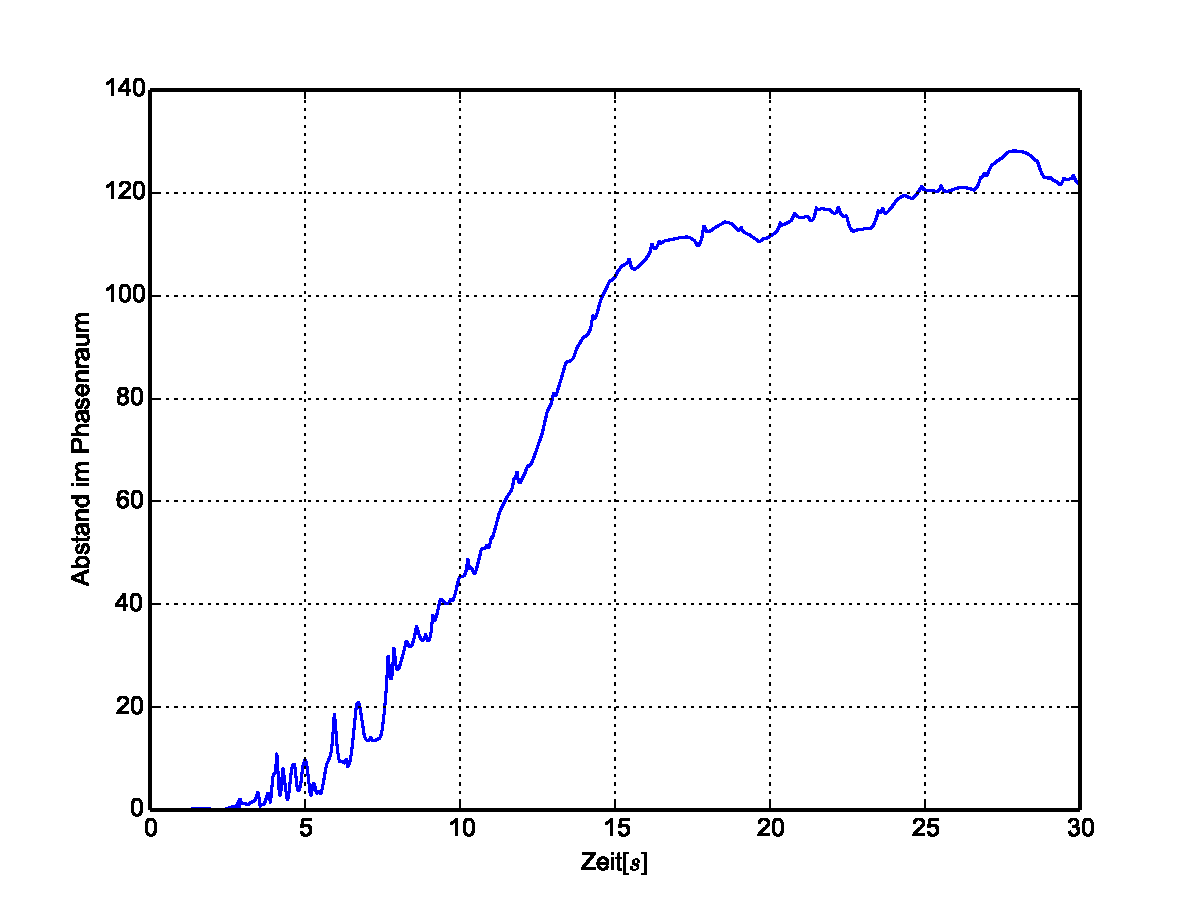
\includegraphics[width = \textwidth]{../Plots/Plot_2_B_2.pdf}
	\caption{Abstand der Trajektorie mit chaotischer Dynamik von derjenigen der ungestörten Schwingung in Abhängigkeit von der Zeit $t$.\label{fig:abstand2}}
\end{figure}
